\documentclass[twoside]{book}

% Packages required by doxygen
\usepackage{fixltx2e}
\usepackage{calc}
\usepackage{doxygen}
\usepackage[export]{adjustbox} % also loads graphicx
\usepackage{graphicx}
\usepackage[utf8]{inputenc}
\usepackage{makeidx}
\usepackage{multicol}
\usepackage{multirow}
\PassOptionsToPackage{warn}{textcomp}
\usepackage{textcomp}
\usepackage[nointegrals]{wasysym}
\usepackage[table]{xcolor}

% Font selection
\usepackage[T1]{fontenc}
\usepackage[scaled=.90]{helvet}
\usepackage{courier}
\usepackage{amssymb}
\usepackage{sectsty}
\renewcommand{\familydefault}{\sfdefault}
\allsectionsfont{%
  \fontseries{bc}\selectfont%
  \color{darkgray}%
}
\renewcommand{\DoxyLabelFont}{%
  \fontseries{bc}\selectfont%
  \color{darkgray}%
}
\newcommand{\+}{\discretionary{\mbox{\scriptsize$\hookleftarrow$}}{}{}}

% Page & text layout
\usepackage{geometry}
\geometry{%
  a4paper,%
  top=2.5cm,%
  bottom=2.5cm,%
  left=2.5cm,%
  right=2.5cm%
}
\tolerance=750
\hfuzz=15pt
\hbadness=750
\setlength{\emergencystretch}{15pt}
\setlength{\parindent}{0cm}
\setlength{\parskip}{3ex plus 2ex minus 2ex}
\makeatletter
\renewcommand{\paragraph}{%
  \@startsection{paragraph}{4}{0ex}{-1.0ex}{1.0ex}{%
    \normalfont\normalsize\bfseries\SS@parafont%
  }%
}
\renewcommand{\subparagraph}{%
  \@startsection{subparagraph}{5}{0ex}{-1.0ex}{1.0ex}{%
    \normalfont\normalsize\bfseries\SS@subparafont%
  }%
}
\makeatother

% Headers & footers
\usepackage{fancyhdr}
\pagestyle{fancyplain}
\fancyhead[LE]{\fancyplain{}{\bfseries\thepage}}
\fancyhead[CE]{\fancyplain{}{}}
\fancyhead[RE]{\fancyplain{}{\bfseries\leftmark}}
\fancyhead[LO]{\fancyplain{}{\bfseries\rightmark}}
\fancyhead[CO]{\fancyplain{}{}}
\fancyhead[RO]{\fancyplain{}{\bfseries\thepage}}
\fancyfoot[LE]{\fancyplain{}{}}
\fancyfoot[CE]{\fancyplain{}{}}
\fancyfoot[RE]{\fancyplain{}{\bfseries\scriptsize Generated by Doxygen }}
\fancyfoot[LO]{\fancyplain{}{\bfseries\scriptsize Generated by Doxygen }}
\fancyfoot[CO]{\fancyplain{}{}}
\fancyfoot[RO]{\fancyplain{}{}}
\renewcommand{\footrulewidth}{0.4pt}
\renewcommand{\chaptermark}[1]{%
  \markboth{#1}{}%
}
\renewcommand{\sectionmark}[1]{%
  \markright{\thesection\ #1}%
}

% Indices & bibliography
\usepackage{natbib}
\usepackage[titles]{tocloft}
\setcounter{tocdepth}{3}
\setcounter{secnumdepth}{5}
\makeindex

% Hyperlinks (required, but should be loaded last)
\usepackage{ifpdf}
\ifpdf
  \usepackage[pdftex,pagebackref=true]{hyperref}
\else
  \usepackage[ps2pdf,pagebackref=true]{hyperref}
\fi
\hypersetup{%
  colorlinks=true,%
  linkcolor=blue,%
  citecolor=blue,%
  unicode%
}

% Custom commands
\newcommand{\clearemptydoublepage}{%
  \newpage{\pagestyle{empty}\cleardoublepage}%
}

\usepackage{caption}
\captionsetup{labelsep=space,justification=centering,font={bf},singlelinecheck=off,skip=4pt,position=top}

%===== C O N T E N T S =====

\begin{document}

% Titlepage & ToC
\hypersetup{pageanchor=false,
             bookmarksnumbered=true,
             pdfencoding=unicode
            }
\pagenumbering{roman}
\begin{titlepage}
\vspace*{7cm}
\begin{center}%
{\Large My Project }\\
\vspace*{1cm}
{\large Generated by Doxygen 1.8.11}\\
\end{center}
\end{titlepage}
\clearemptydoublepage
\tableofcontents
\clearemptydoublepage
\pagenumbering{arabic}
\hypersetup{pageanchor=true}

%--- Begin generated contents ---
\chapter{Class Index}
\section{Class List}
Here are the classes, structs, unions and interfaces with brief descriptions\+:\begin{DoxyCompactList}
\item\contentsline{section}{\hyperlink{structnode}{node} }{\pageref{structnode}}{}
\item\contentsline{section}{\hyperlink{structnode1}{node1} }{\pageref{structnode1}}{}
\item\contentsline{section}{\hyperlink{structnode__info}{node\+\_\+info} }{\pageref{structnode__info}}{}
\end{DoxyCompactList}

\chapter{File Index}
\section{File List}
Here is a list of all files with brief descriptions\+:\begin{DoxyCompactList}
\item\contentsline{section}{\hyperlink{Lab1_8c}{Lab1.\+c} }{\pageref{Lab1_8c}}{}
\end{DoxyCompactList}

\chapter{Class Documentation}
\hypertarget{classArray}{}\section{Array$<$ T $>$ Class Template Reference}
\label{classArray}\index{Array$<$ T $>$@{Array$<$ T $>$}}


{\ttfamily \#include $<$Array.\+h$>$}

\subsection*{Public Member Functions}
\begin{DoxyCompactItemize}
\item 
\hyperlink{classArray_a7503e793980e6d3d5e978fa106a825c2}{Array} (int s=10)
\item 
\hyperlink{classArray_ae9c29e5733413ed09e9137f3c8a71d04}{Array} (const \hyperlink{classArray}{Array}$<$ T $>$ \&)
\item 
\hyperlink{classArray_aab89a85b1ddb86864096acdcc0db439e}{$\sim$\+Array} ()
\item 
const \hyperlink{classArray}{Array}$<$ T $>$ \& \hyperlink{classArray_a0bfa1f9daf4923f45cef66ed086316d7}{operator=} (const \hyperlink{classArray}{Array}$<$ T $>$ \&)
\item 
bool \hyperlink{classArray_ad0fb0f6e80dde0d5e293ae6cfd185ee6}{operator==} (const \hyperlink{classArray}{Array}$<$ T $>$ \&) const 
\item 
bool \hyperlink{classArray_a6f725ca34538a7dc52d097f6c3223a43}{operator!=} (const \hyperlink{classArray}{Array}$<$ T $>$ \&right) const 
\item 
T \& \hyperlink{classArray_a5bae7a87802dbc12faf74956e240c0b2}{operator\mbox{[}$\,$\mbox{]}} (int)
\item 
T \hyperlink{classArray_a0628bf2b0fcd81749659bcc0e2caf0e1}{operator\mbox{[}$\,$\mbox{]}} (int) const 
\item 
int \hyperlink{classArray_a88b824f494fefe7053adf4a5cf55e7cf}{get\+Size} () const 
\item 
T \hyperlink{classArray_aa9850f94775a80016a6ef59e76dac02d}{get\+D\+E\+L\+IM} ()
\item 
void \hyperlink{classArray_aebe3687021d31102a7d52e18bedbffbc}{set\+D\+E\+L\+IM} (T d)
\end{DoxyCompactItemize}
\subsection*{Private Attributes}
\begin{DoxyCompactItemize}
\item 
T \hyperlink{classArray_ab425400868a291283a14fc228a344bf0}{D\+E\+L\+IM}
\item 
int \hyperlink{classArray_a1e2031821065f3fb9bfada13e2d6ab43}{size}
\item 
T $\ast$ \hyperlink{classArray_ae2ca81aaef91da786ef75936184a178a}{d\+Arr}
\end{DoxyCompactItemize}
\subsection*{Static Private Attributes}
\begin{DoxyCompactItemize}
\item 
static const int \hyperlink{classArray_a2fd6afd4cbdf9f82047ec1592d655f9a}{D\+E\+F\+A\+U\+L\+T\+\_\+\+S\+I\+ZE} = 10
\item 
static T \hyperlink{classArray_a0aae993b8d3286cb4e8841cd71e1bb78}{i\+Val}
\end{DoxyCompactItemize}
\subsection*{Friends}
\begin{DoxyCompactItemize}
\item 
ostream \& \hyperlink{classArray_aa67e154869a1f59b76906d7215b7caff}{operator$<$$<$} (ostream \&output, const \hyperlink{classArray}{Array}$<$ T $>$ \&a)
\item 
istream \& \hyperlink{classArray_a6c5c4f2e4fd6da79eec8a53adf3e3f5a}{operator$>$$>$} (istream \&input, \hyperlink{classArray}{Array}$<$ T $>$ \&a)
\end{DoxyCompactItemize}


\subsection{Constructor \& Destructor Documentation}
\index{Array@{Array}!Array@{Array}}
\index{Array@{Array}!Array@{Array}}
\subsubsection[{\texorpdfstring{Array(int s=10)}{Array(int s=10)}}]{\setlength{\rightskip}{0pt plus 5cm}template$<$class T $>$ {\bf Array}$<$ T $>$\+::{\bf Array} (
\begin{DoxyParamCaption}
\item[{int}]{s = {\ttfamily 10}}
\end{DoxyParamCaption}
)}\hypertarget{classArray_a7503e793980e6d3d5e978fa106a825c2}{}\label{classArray_a7503e793980e6d3d5e978fa106a825c2}

\begin{DoxyCode}
21 \{
22    \hyperlink{classArray_a1e2031821065f3fb9bfada13e2d6ab43}{size} = s;
23    \hyperlink{classArray_ae2ca81aaef91da786ef75936184a178a}{dArr} = \textcolor{keyword}{new} \textcolor{keywordtype}{int}[\hyperlink{classArray_a1e2031821065f3fb9bfada13e2d6ab43}{size}];
24 
25    \textcolor{keywordflow}{for} ( \textcolor{keywordtype}{int} i = 0; i < \hyperlink{classArray_a1e2031821065f3fb9bfada13e2d6ab43}{size}; i++ )
26       \hyperlink{classArray_ae2ca81aaef91da786ef75936184a178a}{dArr}[i] = 0;
27 \}
\end{DoxyCode}
\index{Array@{Array}!Array@{Array}}
\index{Array@{Array}!Array@{Array}}
\subsubsection[{\texorpdfstring{Array(const Array$<$ T $>$ \&)}{Array(const Array< T > &)}}]{\setlength{\rightskip}{0pt plus 5cm}template$<$class T $>$ {\bf Array}$<$ T $>$\+::{\bf Array} (
\begin{DoxyParamCaption}
\item[{const {\bf Array}$<$ T $>$ \&}]{array\+To\+Copy}
\end{DoxyParamCaption}
)}\hypertarget{classArray_ae9c29e5733413ed09e9137f3c8a71d04}{}\label{classArray_ae9c29e5733413ed09e9137f3c8a71d04}

\begin{DoxyCode}
36                                        : \hyperlink{classArray_a1e2031821065f3fb9bfada13e2d6ab43}{size}( arrayToCopy.\hyperlink{classArray_a1e2031821065f3fb9bfada13e2d6ab43}{size} )
37 \{
38 
39    \textcolor{comment}{// Copy every element of the passed array to the                                                        
                                                                                                       }
40    \textcolor{comment}{// data member of the array object the function                                                         
                                                                                                       }
41    \textcolor{comment}{// was called on.                                                                                       
                                                                                                       }
42    \hyperlink{classArray_ae2ca81aaef91da786ef75936184a178a}{dArr} = \textcolor{keyword}{new} \textcolor{keywordtype}{int}[\hyperlink{classArray_a1e2031821065f3fb9bfada13e2d6ab43}{size}];
43    \textcolor{keywordflow}{for} ( \textcolor{keywordtype}{int} i = 0; i < \hyperlink{classArray_a1e2031821065f3fb9bfada13e2d6ab43}{size}; i++ )
44       \hyperlink{classArray_ae2ca81aaef91da786ef75936184a178a}{dArr}[i] = arrayToCopy.\hyperlink{classArray_ae2ca81aaef91da786ef75936184a178a}{dArr}[i]; \textcolor{comment}{// copy into object                                           
                                                                                                               }
45 \}
\end{DoxyCode}
\index{Array@{Array}!````~Array@{$\sim$\+Array}}
\index{````~Array@{$\sim$\+Array}!Array@{Array}}
\subsubsection[{\texorpdfstring{$\sim$\+Array()}{~Array()}}]{\setlength{\rightskip}{0pt plus 5cm}template$<$class T $>$ {\bf Array}$<$ T $>$\+::$\sim${\bf Array} (
\begin{DoxyParamCaption}
{}
\end{DoxyParamCaption}
)}\hypertarget{classArray_aab89a85b1ddb86864096acdcc0db439e}{}\label{classArray_aab89a85b1ddb86864096acdcc0db439e}

\begin{DoxyCode}
48 \{
49    \textcolor{keywordflow}{if}(\hyperlink{classArray_ae2ca81aaef91da786ef75936184a178a}{dArr})
50    \{
51       \textcolor{keyword}{delete}[] \hyperlink{classArray_ae2ca81aaef91da786ef75936184a178a}{dArr};\textcolor{comment}{//deletes dynamically allocated memory of array when program ends                  
                                                                                                           }
52       \hyperlink{classArray_ae2ca81aaef91da786ef75936184a178a}{dArr} = NULL;
53    \}
54 \}
\end{DoxyCode}


\subsection{Member Function Documentation}
\index{Array@{Array}!get\+D\+E\+L\+IM@{get\+D\+E\+L\+IM}}
\index{get\+D\+E\+L\+IM@{get\+D\+E\+L\+IM}!Array@{Array}}
\subsubsection[{\texorpdfstring{get\+D\+E\+L\+I\+M()}{getDELIM()}}]{\setlength{\rightskip}{0pt plus 5cm}template$<$class T $>$ T {\bf Array}$<$ T $>$\+::get\+D\+E\+L\+IM (
\begin{DoxyParamCaption}
{}
\end{DoxyParamCaption}
)}\hypertarget{classArray_aa9850f94775a80016a6ef59e76dac02d}{}\label{classArray_aa9850f94775a80016a6ef59e76dac02d}

\begin{DoxyCode}
254 \{
255    \textcolor{keywordflow}{return}( \hyperlink{classArray_ab425400868a291283a14fc228a344bf0}{DELIM} );
256 \}
\end{DoxyCode}
\index{Array@{Array}!get\+Size@{get\+Size}}
\index{get\+Size@{get\+Size}!Array@{Array}}
\subsubsection[{\texorpdfstring{get\+Size() const }{getSize() const }}]{\setlength{\rightskip}{0pt plus 5cm}template$<$class T $>$ int {\bf Array}$<$ T $>$\+::get\+Size (
\begin{DoxyParamCaption}
{}
\end{DoxyParamCaption}
) const}\hypertarget{classArray_a88b824f494fefe7053adf4a5cf55e7cf}{}\label{classArray_a88b824f494fefe7053adf4a5cf55e7cf}

\begin{DoxyCode}
194 \{
195    \textcolor{keywordflow}{return} \hyperlink{classArray_a1e2031821065f3fb9bfada13e2d6ab43}{size}; \textcolor{comment}{// number of elements in Array                                                         
                                                                                                           }
196 \}
\end{DoxyCode}
\index{Array@{Array}!operator"!=@{operator"!=}}
\index{operator"!=@{operator"!=}!Array@{Array}}
\subsubsection[{\texorpdfstring{operator"!=(const Array$<$ T $>$ \&right) const }{operator!=(const Array< T > &right) const }}]{\setlength{\rightskip}{0pt plus 5cm}template$<$class T $>$ bool {\bf Array}$<$ T $>$\+::operator!= (
\begin{DoxyParamCaption}
\item[{const {\bf Array}$<$ T $>$ \&}]{right}
\end{DoxyParamCaption}
) const}\hypertarget{classArray_a6f725ca34538a7dc52d097f6c3223a43}{}\label{classArray_a6f725ca34538a7dc52d097f6c3223a43}

\begin{DoxyCode}
196 \{
197    \textcolor{keywordflow}{return} ! ( *\textcolor{keyword}{this} == right ); \textcolor{comment}{// invokes Array::operator==                                               
                                                                                                       }
198 \}
\end{DoxyCode}


Here is the call graph for this function\+:
\nopagebreak
\begin{figure}[H]
\begin{center}
\leavevmode
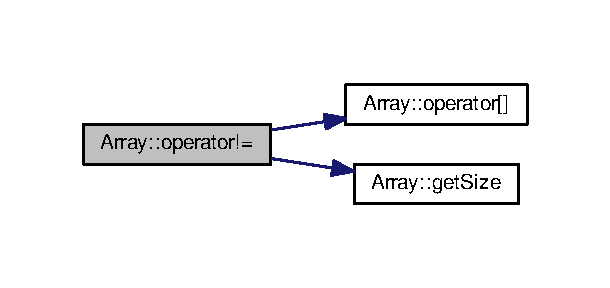
\includegraphics[width=293pt]{classArray_a6f725ca34538a7dc52d097f6c3223a43_cgraph}
\end{center}
\end{figure}


\index{Array@{Array}!operator=@{operator=}}
\index{operator=@{operator=}!Array@{Array}}
\subsubsection[{\texorpdfstring{operator=(const Array$<$ T $>$ \&)}{operator=(const Array< T > &)}}]{\setlength{\rightskip}{0pt plus 5cm}template$<$class T $>$ const {\bf Array}$<$ T $>$ \& {\bf Array}$<$ T $>$\+::operator= (
\begin{DoxyParamCaption}
\item[{const {\bf Array}$<$ T $>$ \&}]{right}
\end{DoxyParamCaption}
)}\hypertarget{classArray_a0bfa1f9daf4923f45cef66ed086316d7}{}\label{classArray_a0bfa1f9daf4923f45cef66ed086316d7}

\begin{DoxyCode}
62 \{
63    \hyperlink{classArray_a1e2031821065f3fb9bfada13e2d6ab43}{size} = right.\hyperlink{classArray_a1e2031821065f3fb9bfada13e2d6ab43}{size};
64 
65    \textcolor{comment}{// Check to see if the arrays are the same object                                                       
                                                                                                       }
66    \textcolor{keywordflow}{if} ( &right != \textcolor{keyword}{this} ) \textcolor{comment}{// this avoids self-assignment                                                    
                                                                                                       }
67    \{
68       \textcolor{keywordflow}{if}(\hyperlink{classArray_ae2ca81aaef91da786ef75936184a178a}{dArr} == NULL)
69       \{
70          cerr << \textcolor{stringliteral}{"Error! Dynamic memory not allocated! Abort program!"} << endl << endl;
71          exit(1);
72       \}
73       \textcolor{keywordflow}{else}
74       \{
75          \textcolor{keyword}{delete}[] \hyperlink{classArray_ae2ca81aaef91da786ef75936184a178a}{dArr};\textcolor{comment}{//delete existing dynamic array so that the new dynamic array can have the right
       size                                                                                                }
76          \hyperlink{classArray_ae2ca81aaef91da786ef75936184a178a}{dArr} = \textcolor{keyword}{new} \textcolor{keywordtype}{int}[\hyperlink{classArray_a1e2031821065f3fb9bfada13e2d6ab43}{size}];
77          \textcolor{keywordflow}{for} ( \textcolor{keywordtype}{int} i = 0; i < \hyperlink{classArray_a1e2031821065f3fb9bfada13e2d6ab43}{size}; i++ )
78             \hyperlink{classArray_ae2ca81aaef91da786ef75936184a178a}{dArr}[i] = right.\hyperlink{classArray_ae2ca81aaef91da786ef75936184a178a}{dArr}[i]; \textcolor{comment}{// copy array into object                                     
                                                                                                               }
79       \}
80    \}
81 
82    \textcolor{keywordflow}{return} *\textcolor{keyword}{this}; \textcolor{comment}{// enables x = y = z                                                                      
                                                                                                       }
83 \}
\end{DoxyCode}
\index{Array@{Array}!operator==@{operator==}}
\index{operator==@{operator==}!Array@{Array}}
\subsubsection[{\texorpdfstring{operator==(const Array$<$ T $>$ \&) const }{operator==(const Array< T > &) const }}]{\setlength{\rightskip}{0pt plus 5cm}template$<$class T $>$ bool {\bf Array}$<$ T $>$\+::operator== (
\begin{DoxyParamCaption}
\item[{const {\bf Array}$<$ T $>$ \&}]{right}
\end{DoxyParamCaption}
) const}\hypertarget{classArray_ad0fb0f6e80dde0d5e293ae6cfd185ee6}{}\label{classArray_ad0fb0f6e80dde0d5e293ae6cfd185ee6}

\begin{DoxyCode}
86 \{
87    \textcolor{keywordtype}{bool} equal = \textcolor{keyword}{true};
88 
89    \textcolor{keywordflow}{if} ( \hyperlink{classArray_a1e2031821065f3fb9bfada13e2d6ab43}{size} != right.\hyperlink{classArray_a1e2031821065f3fb9bfada13e2d6ab43}{size} )
90       equal = \textcolor{keyword}{false}; \textcolor{comment}{// arrays of different number of elements                                             
                                                                                                       }
91    \textcolor{keywordflow}{else}
92       \textcolor{keywordflow}{for} ( \textcolor{keywordtype}{int} i = 0; i < \hyperlink{classArray_a1e2031821065f3fb9bfada13e2d6ab43}{size}; i++ )
93          \textcolor{keywordflow}{if} ( \hyperlink{classArray_ae2ca81aaef91da786ef75936184a178a}{dArr}[i] != right.\hyperlink{classArray_ae2ca81aaef91da786ef75936184a178a}{dArr}[i] )
94          \{
95             equal = \textcolor{keyword}{false}; \textcolor{comment}{// Array contents are not equal, no need to check further                       
                                                                                                       }
96             \textcolor{keywordflow}{break};
97          \}
98    \textcolor{keywordflow}{return}( equal );
99 \}
\end{DoxyCode}
\index{Array@{Array}!operator\mbox{[}$\,$\mbox{]}@{operator[]}}
\index{operator\mbox{[}$\,$\mbox{]}@{operator[]}!Array@{Array}}
\subsubsection[{\texorpdfstring{operator[](int)}{operator[](int)}}]{\setlength{\rightskip}{0pt plus 5cm}template$<$class T $>$ T \& {\bf Array}$<$ T $>$\+::operator\mbox{[}$\,$\mbox{]} (
\begin{DoxyParamCaption}
\item[{int}]{subscript}
\end{DoxyParamCaption}
)}\hypertarget{classArray_a5bae7a87802dbc12faf74956e240c0b2}{}\label{classArray_a5bae7a87802dbc12faf74956e240c0b2}

\begin{DoxyCode}
110 \{
111    \textcolor{comment}{// check for subscript out-of-range error                                                               
                                                                                                       }
112    \textcolor{comment}{//                                                                                                      
                                                                                                       }
113    \textcolor{comment}{// this is an unrecoverable error so without exception handling,                                        
                                                                                                       }
114    \textcolor{comment}{// program can only log the error and exit.                                                             
                                                                                                       }
115    \textcolor{keywordflow}{if} ( subscript < 0 || (subscript >= \hyperlink{classArray_a1e2031821065f3fb9bfada13e2d6ab43}{size}) )
116    \{
117       cerr << \textcolor{stringliteral}{"\(\backslash\)nError: Subscript "} << subscript
118            << \textcolor{stringliteral}{" out of range, exiting program"} << endl;
119       exit( 1 ); \textcolor{comment}{// terminate program; subscript out of range  }
120    \}
121 
122    \textcolor{keywordflow}{return} \hyperlink{classArray_ae2ca81aaef91da786ef75936184a178a}{dArr}[subscript]; \textcolor{comment}{// reference return so returning address location not contents              
                                                                                                           }
123 \}
\end{DoxyCode}
\index{Array@{Array}!operator\mbox{[}$\,$\mbox{]}@{operator[]}}
\index{operator\mbox{[}$\,$\mbox{]}@{operator[]}!Array@{Array}}
\subsubsection[{\texorpdfstring{operator[](int) const }{operator[](int) const }}]{\setlength{\rightskip}{0pt plus 5cm}template$<$class T $>$ T {\bf Array}$<$ T $>$\+::operator\mbox{[}$\,$\mbox{]} (
\begin{DoxyParamCaption}
\item[{int}]{subscript}
\end{DoxyParamCaption}
) const}\hypertarget{classArray_a0628bf2b0fcd81749659bcc0e2caf0e1}{}\label{classArray_a0628bf2b0fcd81749659bcc0e2caf0e1}

\begin{DoxyCode}
131 \{
132    \textcolor{comment}{// check for subscript out-of-range error                                                               
                                                                                                       }
133    \textcolor{keywordflow}{if} ( subscript < 0 || subscript >= \hyperlink{classArray_a1e2031821065f3fb9bfada13e2d6ab43}{size} )
134    \{
135       cerr << \textcolor{stringliteral}{"\(\backslash\)nError: Subscript "} << subscript
136            << \textcolor{stringliteral}{" out of range, exiting program"} << endl;
137       exit( 1 ); \textcolor{comment}{// terminate program; subscript out of range                                              
                                                                                                       }
138    \}
139 
140    \textcolor{keywordflow}{return} \hyperlink{classArray_ae2ca81aaef91da786ef75936184a178a}{dArr}[subscript]; \textcolor{comment}{// returns copy of this element and not the address location                
                                                                                                           }
141 \}
\end{DoxyCode}
\index{Array@{Array}!set\+D\+E\+L\+IM@{set\+D\+E\+L\+IM}}
\index{set\+D\+E\+L\+IM@{set\+D\+E\+L\+IM}!Array@{Array}}
\subsubsection[{\texorpdfstring{set\+D\+E\+L\+I\+M(\+T d)}{setDELIM(T d)}}]{\setlength{\rightskip}{0pt plus 5cm}template$<$class T $>$ void {\bf Array}$<$ T $>$\+::set\+D\+E\+L\+IM (
\begin{DoxyParamCaption}
\item[{T}]{d}
\end{DoxyParamCaption}
)}\hypertarget{classArray_aebe3687021d31102a7d52e18bedbffbc}{}\label{classArray_aebe3687021d31102a7d52e18bedbffbc}

\begin{DoxyCode}
260 \{
261    \hyperlink{classArray_ab425400868a291283a14fc228a344bf0}{DELIM} = d;
262 \}
\end{DoxyCode}


\subsection{Friends And Related Function Documentation}
\index{Array@{Array}!operator$<$$<$@{operator$<$$<$}}
\index{operator$<$$<$@{operator$<$$<$}!Array@{Array}}
\subsubsection[{\texorpdfstring{operator$<$$<$}{operator<<}}]{\setlength{\rightskip}{0pt plus 5cm}template$<$class T$>$ ostream\& operator$<$$<$ (
\begin{DoxyParamCaption}
\item[{ostream \&}]{output, }
\item[{const {\bf Array}$<$ T $>$ \&}]{a}
\end{DoxyParamCaption}
)\hspace{0.3cm}{\ttfamily [friend]}}\hypertarget{classArray_aa67e154869a1f59b76906d7215b7caff}{}\label{classArray_aa67e154869a1f59b76906d7215b7caff}

\begin{DoxyCode}
24    \{
25       \textcolor{keywordtype}{int} i;
26 
27       cout << endl;
28 
29       \textcolor{comment}{// output private ptr-based array                                                                    
                                                                                                       }
30       \textcolor{keywordflow}{for} ( i = 0; i < a.\hyperlink{classArray_a1e2031821065f3fb9bfada13e2d6ab43}{size}; i++ )
31       \{
32          output << right << setw(10) << a.\hyperlink{classArray_ae2ca81aaef91da786ef75936184a178a}{dArr}[i];
33 
34          \textcolor{keywordflow}{if} ( (i + 1) % 4 == 0 ) \textcolor{comment}{// 4 numbers per row of output                                            
                                                                                                       }
35             output << endl;
36       \}
37 
38       \textcolor{keywordflow}{if} ( i % 4 != 0 ) \textcolor{comment}{// end last line of output                                                         
                                                                                                       }
39          output << endl;
40 
41       \textcolor{keywordflow}{return} output; \textcolor{comment}{// enables cout << x << y;                                                            
                                                                                                       }
42    \}
\end{DoxyCode}
\index{Array@{Array}!operator$>$$>$@{operator$>$$>$}}
\index{operator$>$$>$@{operator$>$$>$}!Array@{Array}}
\subsubsection[{\texorpdfstring{operator$>$$>$}{operator>>}}]{\setlength{\rightskip}{0pt plus 5cm}template$<$class T$>$ istream\& operator$>$$>$ (
\begin{DoxyParamCaption}
\item[{istream \&}]{input, }
\item[{{\bf Array}$<$ T $>$ \&}]{a}
\end{DoxyParamCaption}
)\hspace{0.3cm}{\ttfamily [friend]}}\hypertarget{classArray_a6c5c4f2e4fd6da79eec8a53adf3e3f5a}{}\label{classArray_a6c5c4f2e4fd6da79eec8a53adf3e3f5a}

\begin{DoxyCode}
45    \{
46       vector<T> v;
47       T t;
48       input >> t;
49 
50       \textcolor{keywordflow}{while}(t != a.\hyperlink{classArray_ab425400868a291283a14fc228a344bf0}{DELIM})\textcolor{comment}{//takes in all the integers entered up until DELIM is entered                
                                                                                                            }
51       \{
52          v.push\_back(t); \textcolor{comment}{//adds the element entered to the vector                                          
                                                                                                       }
53          input >> t;
54       \}
55 
56       \hyperlink{classArray}{Array<T>} b(v.size()); \textcolor{comment}{//initializes the array with the size of vector v                      
                                                                                                               }
57       \textcolor{keywordflow}{if}(b.dArr == NULL) \textcolor{comment}{//if b's dynamic array has no memory allocated                                    
                                                                                                       }
58       \{
59          cerr << \textcolor{stringliteral}{"Error! Dynamic memory not allocated! Abort program!"} << endl << endl;
60          exit(1);
61       \}
62 
63       \textcolor{keywordflow}{for}(\textcolor{keywordtype}{int} k=0; k<b.size; k++)
64          b.dArr[k] = v[k]; \textcolor{comment}{//assigning the values in the vector to the newly created dynamic array         
                                                                                                       }
65 
66       a = b; \textcolor{comment}{//assign b to a                                                                               
                                                                                                       }
67       return (input); \textcolor{comment}{// enables cin >> x >> y;                                                            
                                                                                                       }
68    \}
\end{DoxyCode}


\subsection{Member Data Documentation}
\index{Array@{Array}!d\+Arr@{d\+Arr}}
\index{d\+Arr@{d\+Arr}!Array@{Array}}
\subsubsection[{\texorpdfstring{d\+Arr}{dArr}}]{\setlength{\rightskip}{0pt plus 5cm}template$<$class T$>$ T$\ast$ {\bf Array}$<$ T $>$\+::d\+Arr\hspace{0.3cm}{\ttfamily [private]}}\hypertarget{classArray_ae2ca81aaef91da786ef75936184a178a}{}\label{classArray_ae2ca81aaef91da786ef75936184a178a}
\index{Array@{Array}!D\+E\+F\+A\+U\+L\+T\+\_\+\+S\+I\+ZE@{D\+E\+F\+A\+U\+L\+T\+\_\+\+S\+I\+ZE}}
\index{D\+E\+F\+A\+U\+L\+T\+\_\+\+S\+I\+ZE@{D\+E\+F\+A\+U\+L\+T\+\_\+\+S\+I\+ZE}!Array@{Array}}
\subsubsection[{\texorpdfstring{D\+E\+F\+A\+U\+L\+T\+\_\+\+S\+I\+ZE}{DEFAULT_SIZE}}]{\setlength{\rightskip}{0pt plus 5cm}template$<$class T$>$ const int {\bf Array}$<$ T $>$\+::D\+E\+F\+A\+U\+L\+T\+\_\+\+S\+I\+ZE = 10\hspace{0.3cm}{\ttfamily [static]}, {\ttfamily [private]}}\hypertarget{classArray_a2fd6afd4cbdf9f82047ec1592d655f9a}{}\label{classArray_a2fd6afd4cbdf9f82047ec1592d655f9a}
\index{Array@{Array}!D\+E\+L\+IM@{D\+E\+L\+IM}}
\index{D\+E\+L\+IM@{D\+E\+L\+IM}!Array@{Array}}
\subsubsection[{\texorpdfstring{D\+E\+L\+IM}{DELIM}}]{\setlength{\rightskip}{0pt plus 5cm}template$<$class T$>$ T {\bf Array}$<$ T $>$\+::D\+E\+L\+IM\hspace{0.3cm}{\ttfamily [private]}}\hypertarget{classArray_ab425400868a291283a14fc228a344bf0}{}\label{classArray_ab425400868a291283a14fc228a344bf0}
\index{Array@{Array}!i\+Val@{i\+Val}}
\index{i\+Val@{i\+Val}!Array@{Array}}
\subsubsection[{\texorpdfstring{i\+Val}{iVal}}]{\setlength{\rightskip}{0pt plus 5cm}template$<$class T$>$ T {\bf Array}$<$ T $>$\+::i\+Val\hspace{0.3cm}{\ttfamily [static]}, {\ttfamily [private]}}\hypertarget{classArray_a0aae993b8d3286cb4e8841cd71e1bb78}{}\label{classArray_a0aae993b8d3286cb4e8841cd71e1bb78}
\index{Array@{Array}!size@{size}}
\index{size@{size}!Array@{Array}}
\subsubsection[{\texorpdfstring{size}{size}}]{\setlength{\rightskip}{0pt plus 5cm}template$<$class T$>$ int {\bf Array}$<$ T $>$\+::size\hspace{0.3cm}{\ttfamily [private]}}\hypertarget{classArray_a1e2031821065f3fb9bfada13e2d6ab43}{}\label{classArray_a1e2031821065f3fb9bfada13e2d6ab43}


The documentation for this class was generated from the following files\+:\begin{DoxyCompactItemize}
\item 
\hyperlink{Array_8h}{Array.\+h}\item 
\hyperlink{Array_8cpp}{Array.\+cpp}\end{DoxyCompactItemize}

\chapter{File Documentation}
\hypertarget{Amain_8cpp}{}\section{Amain.\+cpp File Reference}
\label{Amain_8cpp}\index{Amain.\+cpp@{Amain.\+cpp}}
{\ttfamily \#include $<$iostream$>$}\\*
{\ttfamily \#include \char`\"{}Account.\+h\char`\"{}}\\*
Include dependency graph for Amain.\+cpp\+:
\nopagebreak
\begin{figure}[H]
\begin{center}
\leavevmode
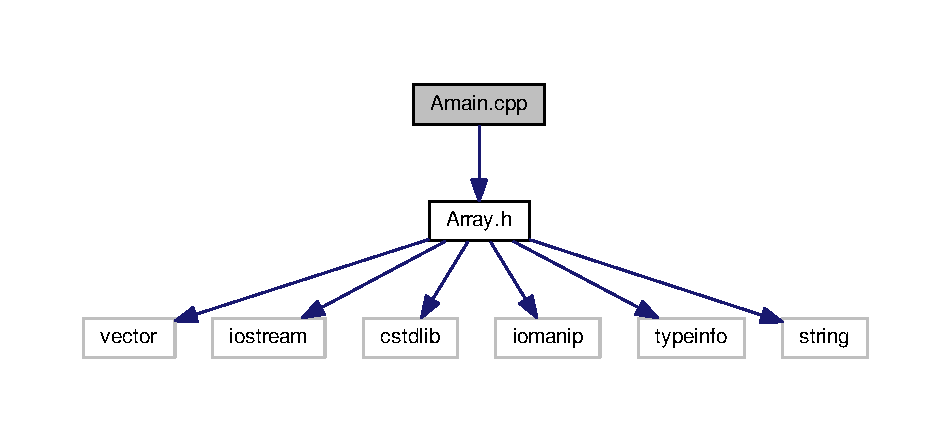
\includegraphics[width=214pt]{Amain_8cpp__incl}
\end{center}
\end{figure}
\subsection*{Functions}
\begin{DoxyCompactItemize}
\item 
int \hyperlink{Amain_8cpp_ae66f6b31b5ad750f1fe042a706a4e3d4}{main} ()
\end{DoxyCompactItemize}


\subsection{Function Documentation}
\index{Amain.\+cpp@{Amain.\+cpp}!main@{main}}
\index{main@{main}!Amain.\+cpp@{Amain.\+cpp}}
\subsubsection[{\texorpdfstring{main()}{main()}}]{\setlength{\rightskip}{0pt plus 5cm}int main (
\begin{DoxyParamCaption}
{}
\end{DoxyParamCaption}
)}\hypertarget{Amain_8cpp_ae66f6b31b5ad750f1fe042a706a4e3d4}{}\label{Amain_8cpp_ae66f6b31b5ad750f1fe042a706a4e3d4}

\begin{DoxyCode}
7            \{
8     \hyperlink{classAccount}{Account} a1(8111, 99.99);
9     a1.print();     \textcolor{comment}{// A/C no: 8111 Balance=$99.99}
10     a1.credit(20);
11     a1.debit(10);
12     a1.print();     \textcolor{comment}{// A/C no: 8111 Balance=$109.99}
13  
14     \hyperlink{classAccount}{Account} a2(8222);  \textcolor{comment}{// default balance}
15     a2.print();        \textcolor{comment}{// A/C no: 8222 Balance=$0.00}
16     a2.setBalance(100);
17     a2.credit(20);
18     a2.debit(200);  \textcolor{comment}{// Amount withdrawn exceeds the current balance!}
19     a2.print();     \textcolor{comment}{// A/C no: 8222 Balance=$120.00}
20     \textcolor{keywordflow}{return} 0;
21 \}\end{DoxyCode}


Here is the call graph for this function\+:
\nopagebreak
\begin{figure}[H]
\begin{center}
\leavevmode
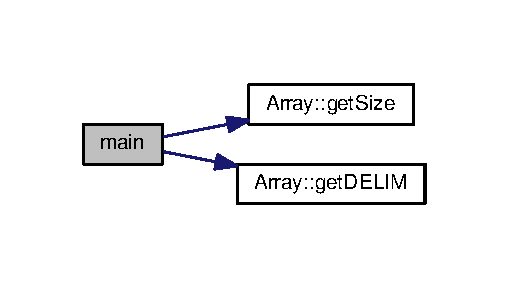
\includegraphics[width=350pt]{Amain_8cpp_ae66f6b31b5ad750f1fe042a706a4e3d4_cgraph}
\end{center}
\end{figure}



\hypertarget{Amain2_8cpp}{}\section{Amain2.\+cpp File Reference}
\label{Amain2_8cpp}\index{Amain2.\+cpp@{Amain2.\+cpp}}
{\ttfamily \#include \char`\"{}Array.\+h\char`\"{}}\\*
Include dependency graph for Amain2.\+cpp\+:
\nopagebreak
\begin{figure}[H]
\begin{center}
\leavevmode
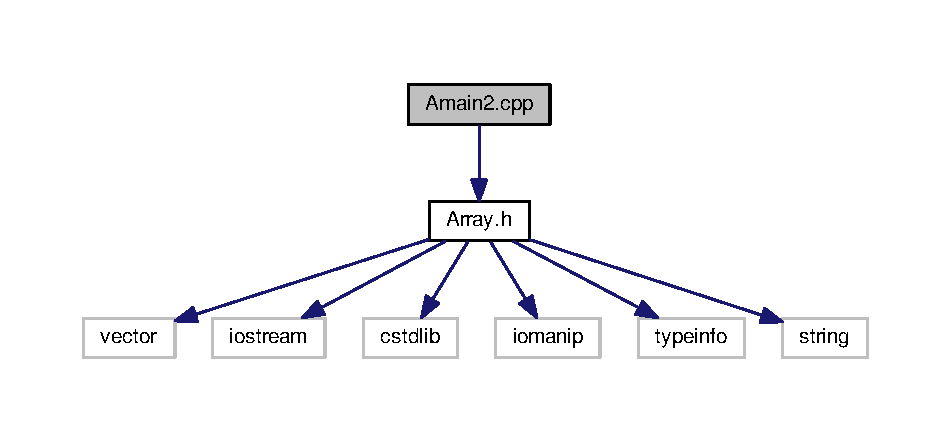
\includegraphics[width=350pt]{Amain2_8cpp__incl}
\end{center}
\end{figure}
\subsection*{Functions}
\begin{DoxyCompactItemize}
\item 
{\footnotesize template$<$typename T $>$ }\\void \hyperlink{Amain2_8cpp_a3314cbbca00e99ccc8b9d46dce272b0d}{instantiate\+Array} (\hyperlink{classArray}{Array}$<$ T $>$ \&a)
\item 
int \hyperlink{Amain2_8cpp_ae66f6b31b5ad750f1fe042a706a4e3d4}{main} ()
\end{DoxyCompactItemize}


\subsection{Function Documentation}
\index{Amain2.\+cpp@{Amain2.\+cpp}!instantiate\+Array@{instantiate\+Array}}
\index{instantiate\+Array@{instantiate\+Array}!Amain2.\+cpp@{Amain2.\+cpp}}
\subsubsection[{\texorpdfstring{instantiate\+Array(\+Array$<$ T $>$ \&a)}{instantiateArray(Array< T > &a)}}]{\setlength{\rightskip}{0pt plus 5cm}template$<$typename T $>$ void instantiate\+Array (
\begin{DoxyParamCaption}
\item[{{\bf Array}$<$ T $>$ \&}]{a}
\end{DoxyParamCaption}
)}\hypertarget{Amain2_8cpp_a3314cbbca00e99ccc8b9d46dce272b0d}{}\label{Amain2_8cpp_a3314cbbca00e99ccc8b9d46dce272b0d}

\begin{DoxyCode}
44 \{
45    \textcolor{keyword}{static} T dVal; \textcolor{comment}{//is initialized with a default T value                                                  
                                                                                                       }
46 
47    cout << \textcolor{stringliteral}{"\(\backslash\)nEnter any amount of elements or "} << a.\hyperlink{classArray_aa9850f94775a80016a6ef59e76dac02d}{getDELIM}() << \textcolor{stringliteral}{" to end input: "};
48    cin >> a;
49    cout << a.\hyperlink{classArray_a88b824f494fefe7053adf4a5cf55e7cf}{getSize}() << \textcolor{stringliteral}{" elements were entered\(\backslash\)n"} << a << endl;
50 
51    cout << \textcolor{stringliteral}{"Initializing second array from the array originally created"} << endl;
52    \hyperlink{classArray}{Array<T>} b(a); \textcolor{comment}{//initializing a new array as a copy of the original                             
                                                                                                               }
53    cout << \textcolor{stringliteral}{"the new array has "} << b.getSize() << \textcolor{stringliteral}{" elements\(\backslash\)n"} << b << endl;
54 
55    cout << \textcolor{stringliteral}{"The original array and second array are "};
56    \textcolor{keywordflow}{if}(a==b) \textcolor{comment}{//checks to see if a and b are the same arrays                                                 
                                                                                                       }
57       cout << \textcolor{stringliteral}{"equal"} << endl;
58    \textcolor{keywordflow}{else}
59       cout << \textcolor{stringliteral}{"not equal"} << endl;
60 
61    cout << \textcolor{stringliteral}{"Creating a third array from user input..."};
62    \hyperlink{classArray}{Array<T>} c; \textcolor{comment}{//creates default array c of the same type as array a                               
                                                                                                               }
63    c.\hyperlink{classArray_aebe3687021d31102a7d52e18bedbffbc}{setDELIM}(a.getDELIM()); \textcolor{comment}{//sets the DELIM of c to the same as a                                
                                                                                                               }
64    cout << \textcolor{stringliteral}{"\(\backslash\)nEnter any amount of elements or "} << c.\hyperlink{classArray_aa9850f94775a80016a6ef59e76dac02d}{getDELIM}() << \textcolor{stringliteral}{" to end input: "};
65    cin >> c;
66    cout << c.\hyperlink{classArray_a88b824f494fefe7053adf4a5cf55e7cf}{getSize}() << \textcolor{stringliteral}{" elements were entered\(\backslash\)n"} << c << endl;
67 
68    cout << \textcolor{stringliteral}{"The original array and third array are "};
69    \textcolor{keywordflow}{if}(a==c) \textcolor{comment}{//checks if a and c are the same array                                                         
                                                                                                       }
70       cout << \textcolor{stringliteral}{"equal"} << endl;
71    \textcolor{keywordflow}{else}
72       cout << \textcolor{stringliteral}{"not equal"} << endl;
73 
74    cout << \textcolor{stringliteral}{"Copying the elements from the third array to the original one"} << endl;
75    a = c; \textcolor{comment}{//copies the array of c to a                                                                     
                                                                                                       }
76    cout << \textcolor{stringliteral}{"The original array now has "} << a.getSize() << \textcolor{stringliteral}{" elements:\(\backslash\)n"} << a << endl;
77 
78    \textcolor{comment}{//uses overloaded subscript operator to print out value at a[5]                                         
                                                                                                       }
79    cout << \textcolor{stringliteral}{"In the original array, the element at subscript 5 is "} << a[5] << endl;
80 
81    \textcolor{comment}{// use overloaded subscript operator to create lvalue                                                   
                                                                                                       }
82    cout << \textcolor{stringliteral}{"\(\backslash\)n\(\backslash\)nAssigning "} << dVal << \textcolor{stringliteral}{" to the subscript [5] position"} << endl;
83    a[ 5 ] = dVal; \textcolor{comment}{//a[5] is assigned dVal's value                                                          
                                                                                                       }
84    cout << \textcolor{stringliteral}{"After assignment, the original array:\(\backslash\)n"} << a << endl;
85 \}
\end{DoxyCode}


Here is the call graph for this function\+:
\nopagebreak
\begin{figure}[H]
\begin{center}
\leavevmode
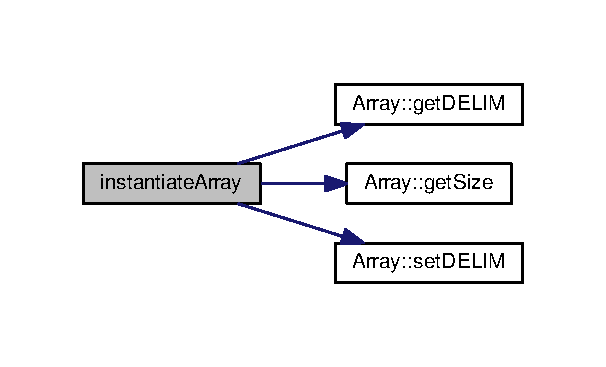
\includegraphics[width=291pt]{Amain2_8cpp_a3314cbbca00e99ccc8b9d46dce272b0d_cgraph}
\end{center}
\end{figure}


\index{Amain2.\+cpp@{Amain2.\+cpp}!main@{main}}
\index{main@{main}!Amain2.\+cpp@{Amain2.\+cpp}}
\subsubsection[{\texorpdfstring{main()}{main()}}]{\setlength{\rightskip}{0pt plus 5cm}int main (
\begin{DoxyParamCaption}
{}
\end{DoxyParamCaption}
)}\hypertarget{Amain2_8cpp_ae66f6b31b5ad750f1fe042a706a4e3d4}{}\label{Amain2_8cpp_ae66f6b31b5ad750f1fe042a706a4e3d4}

\begin{DoxyCode}
14 \{
15    \textcolor{comment}{// Instantiate an Array of doubles                                                                      
                                                                                                       }
16    cout << \textcolor{stringliteral}{"\(\backslash\)nTESTING DOUBLES:\(\backslash\)n"};
17    \hyperlink{classArray}{Array<double>} dbl;
18    dbl.\hyperlink{classArray_aebe3687021d31102a7d52e18bedbffbc}{setDELIM}(-999); \textcolor{comment}{//sets the DELIM based on Array type for input purposes                     
                                                                                                               }
19    \hyperlink{Amain2_8cpp_a3314cbbca00e99ccc8b9d46dce272b0d}{instantiateArray}(dbl);
20 
21    \textcolor{comment}{// Instantiate an Array of integers                                                                     
                                                                                                       }
22    cout << \textcolor{stringliteral}{"\(\backslash\)nTESTING INTEGERS:\(\backslash\)n"};
23    \hyperlink{classArray}{Array<int>} i;
24    i.\hyperlink{classArray_aebe3687021d31102a7d52e18bedbffbc}{setDELIM}(-999);
25    \hyperlink{Amain2_8cpp_a3314cbbca00e99ccc8b9d46dce272b0d}{instantiateArray}(i);
26 
27    \textcolor{comment}{// Instantiate an Array of characters                                                                   
                                                                                                       }
28    cout << \textcolor{stringliteral}{"\(\backslash\)nTESTING CHARS:\(\backslash\)n"};
29    \hyperlink{classArray}{Array<char>} c;
30    c.\hyperlink{classArray_aebe3687021d31102a7d52e18bedbffbc}{setDELIM}(\textcolor{charliteral}{'*'});
31    \hyperlink{Amain2_8cpp_a3314cbbca00e99ccc8b9d46dce272b0d}{instantiateArray}(c);
32 
33    \textcolor{comment}{// Instantiate an Array of strings                                                                      
                                                                                                       }
34    cout << \textcolor{stringliteral}{"\(\backslash\)nTESTING STRINGS:\(\backslash\)n"};
35    \hyperlink{classArray}{Array<string>} s;
36    s.\hyperlink{classArray_aebe3687021d31102a7d52e18bedbffbc}{setDELIM}(\textcolor{stringliteral}{"-999"});
37    \hyperlink{Amain2_8cpp_a3314cbbca00e99ccc8b9d46dce272b0d}{instantiateArray}(s);
38 
39    \textcolor{keywordflow}{return} 0;
40 \}
\end{DoxyCode}


Here is the call graph for this function\+:
\nopagebreak
\begin{figure}[H]
\begin{center}
\leavevmode
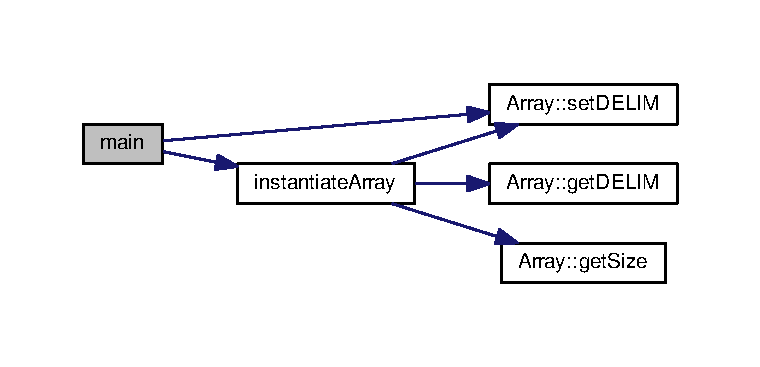
\includegraphics[width=350pt]{Amain2_8cpp_ae66f6b31b5ad750f1fe042a706a4e3d4_cgraph}
\end{center}
\end{figure}



\hypertarget{Array_8cpp}{}\section{Array.\+cpp File Reference}
\label{Array_8cpp}\index{Array.\+cpp@{Array.\+cpp}}
{\ttfamily \#include \char`\"{}Array.\+h\char`\"{}}\\*
Include dependency graph for Array.\+cpp\+:
\nopagebreak
\begin{figure}[H]
\begin{center}
\leavevmode
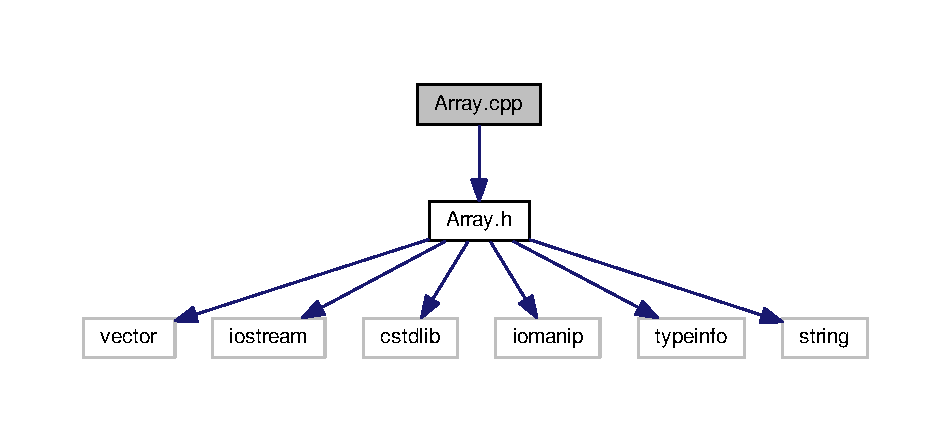
\includegraphics[width=350pt]{Array_8cpp__incl}
\end{center}
\end{figure}
\subsection*{Functions}
\begin{DoxyCompactItemize}
\item 
istream \& \hyperlink{Array_8cpp_a14edf7ce8faebaaec1b5e81582fed73b}{operator$>$$>$} (istream \&input, \hyperlink{classArray}{Array} \&a)
\item 
ostream \& \hyperlink{Array_8cpp_a37415f259690744fe14f0589d4e74fb7}{operator$<$$<$} (ostream \&output, const \hyperlink{classArray}{Array} \&a)
\end{DoxyCompactItemize}


\subsection{Function Documentation}
\index{Array.\+cpp@{Array.\+cpp}!operator$<$$<$@{operator$<$$<$}}
\index{operator$<$$<$@{operator$<$$<$}!Array.\+cpp@{Array.\+cpp}}
\subsubsection[{\texorpdfstring{operator$<$$<$(ostream \&output, const Array \&a)}{operator<<(ostream &output, const Array &a)}}]{\setlength{\rightskip}{0pt plus 5cm}ostream\& operator$<$$<$ (
\begin{DoxyParamCaption}
\item[{ostream \&}]{output, }
\item[{const {\bf Array} \&}]{a}
\end{DoxyParamCaption}
)}\hypertarget{Array_8cpp_a37415f259690744fe14f0589d4e74fb7}{}\label{Array_8cpp_a37415f259690744fe14f0589d4e74fb7}

\begin{DoxyCode}
172 \{
173    \textcolor{keywordtype}{int} i;
174 
175    cout << endl;
176 
177    \textcolor{comment}{// output private ptr-based array                                                                       
                                                                                                       }
178    \textcolor{keywordflow}{for} ( i = 0; i < a.\hyperlink{classArray_a1e2031821065f3fb9bfada13e2d6ab43}{size}; i++ )
179    \{
180       output << right << setw(10) << a.\hyperlink{classArray_ae2ca81aaef91da786ef75936184a178a}{dArr}[i];
181 
182       \textcolor{keywordflow}{if} ( (i + 1) % 4 == 0 ) \textcolor{comment}{// 4 numbers per row of output                                               
                                                                                                       }
183          output << endl;
184    \}
185 
186    \textcolor{keywordflow}{if} ( i % 4 != 0 ) \textcolor{comment}{// end last line of output                                                            
                                                                                                       }
187       output << endl;
188 
189    \textcolor{keywordflow}{return} output; \textcolor{comment}{// enables cout << x << y;                                                               
                                                                                                       }
190 \}
\end{DoxyCode}
\index{Array.\+cpp@{Array.\+cpp}!operator$>$$>$@{operator$>$$>$}}
\index{operator$>$$>$@{operator$>$$>$}!Array.\+cpp@{Array.\+cpp}}
\subsubsection[{\texorpdfstring{operator$>$$>$(istream \&input, Array \&a)}{operator>>(istream &input, Array &a)}}]{\setlength{\rightskip}{0pt plus 5cm}istream\& operator$>$$>$ (
\begin{DoxyParamCaption}
\item[{istream \&}]{input, }
\item[{{\bf Array} \&}]{a}
\end{DoxyParamCaption}
)}\hypertarget{Array_8cpp_a14edf7ce8faebaaec1b5e81582fed73b}{}\label{Array_8cpp_a14edf7ce8faebaaec1b5e81582fed73b}

\begin{DoxyCode}
146 \{
147    vector<int> v;
148    \textcolor{keywordtype}{int} c;
149 
150    input >> c;
151    \textcolor{keywordflow}{while}(c != \hyperlink{classArray_ab425400868a291283a14fc228a344bf0}{Array::DELIM})\textcolor{comment}{//takes in all the integers entered up until DELIM is entered       
                                                                                                                  
       }
152    \{
153       v.push\_back(c);
154       input >> c;
155    \}
156 
157    \hyperlink{classArray}{Array} b(v.size());
158    \textcolor{keywordflow}{if}(b.dArr == NULL)
159    \{
160       cerr << \textcolor{stringliteral}{"Error! Dynamic memory not allocated! Abort program!"} << endl << endl;
161       exit(1);
162    \}
163 
164    \textcolor{keywordflow}{for}(\textcolor{keywordtype}{int} k=0; k<b.size; k++)
165       b.dArr[k] = v[k];
166 
167    a = b;
168    return (input); \textcolor{comment}{// enables cin >> x >> y;                                                               
                                                                                                       }
169 \}
\end{DoxyCode}

\hypertarget{Array_8h}{}\section{Array.\+h File Reference}
\label{Array_8h}\index{Array.\+h@{Array.\+h}}
{\ttfamily \#include $<$vector$>$}\\*
{\ttfamily \#include $<$iostream$>$}\\*
{\ttfamily \#include $<$cstdlib$>$}\\*
{\ttfamily \#include $<$iomanip$>$}\\*
{\ttfamily \#include $<$typeinfo$>$}\\*
{\ttfamily \#include $<$string$>$}\\*
Include dependency graph for Array.\+h\+:
\nopagebreak
\begin{figure}[H]
\begin{center}
\leavevmode
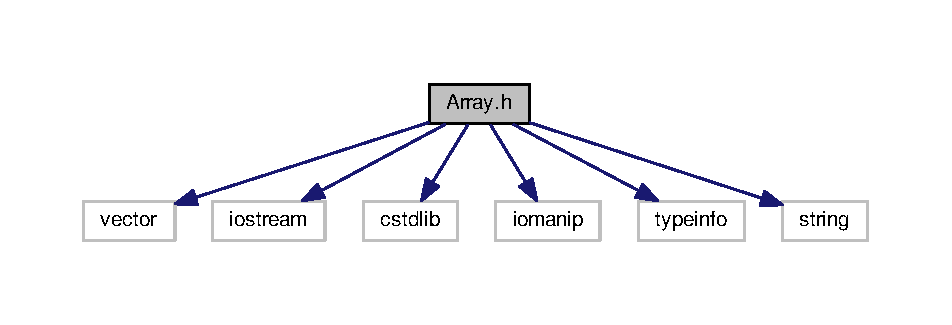
\includegraphics[width=350pt]{Array_8h__incl}
\end{center}
\end{figure}
This graph shows which files directly or indirectly include this file\+:
\nopagebreak
\begin{figure}[H]
\begin{center}
\leavevmode
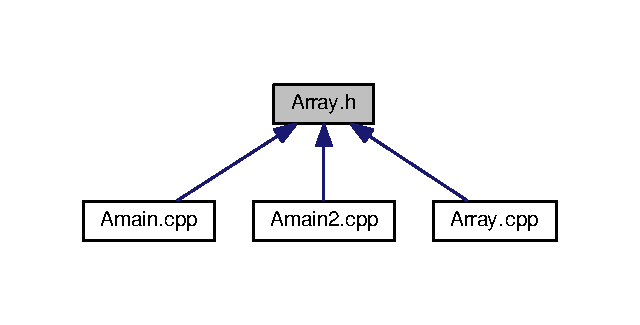
\includegraphics[width=307pt]{Array_8h__dep__incl}
\end{center}
\end{figure}
\subsection*{Classes}
\begin{DoxyCompactItemize}
\item 
class \hyperlink{classArray}{Array$<$ T $>$}
\end{DoxyCompactItemize}
\subsection*{Macros}
\begin{DoxyCompactItemize}
\item 
\#define \hyperlink{Array_8h_ac6905e5d185c7e5990c56ececee8d8e5}{A\+R\+R\+A\+Y\+\_\+H}
\end{DoxyCompactItemize}


\subsection{Macro Definition Documentation}
\index{Array.\+h@{Array.\+h}!A\+R\+R\+A\+Y\+\_\+H@{A\+R\+R\+A\+Y\+\_\+H}}
\index{A\+R\+R\+A\+Y\+\_\+H@{A\+R\+R\+A\+Y\+\_\+H}!Array.\+h@{Array.\+h}}
\subsubsection[{\texorpdfstring{A\+R\+R\+A\+Y\+\_\+H}{ARRAY_H}}]{\setlength{\rightskip}{0pt plus 5cm}\#define A\+R\+R\+A\+Y\+\_\+H}\hypertarget{Array_8h_ac6905e5d185c7e5990c56ececee8d8e5}{}\label{Array_8h_ac6905e5d185c7e5990c56ececee8d8e5}

%--- End generated contents ---

% Index
\backmatter
\newpage
\phantomsection
\clearemptydoublepage
\addcontentsline{toc}{chapter}{Index}
\printindex

\end{document}
